\documentclass[12pt]{beamer}
\usetheme{metropolis}           % Use metropolis theme
\metroset{titleformat=smallcaps}

\usepackage[utf8]{inputenc}
\usepackage[T1]{fontenc}
\usepackage{textcomp}
% \usepackage{amsmath,amsfonts,amssymb}
\usepackage{url}

% disable Navigation at the bottom
\beamertemplatenavigationsymbolsempty

% Cool font
\usepackage{FiraSans}
% \usepackage[sfdefault,light]{FiraSans}
% \usepackage{newtxsf}

% page numbers
% \setbeamertemplate{footline}[frame number]
% \setbeamertemplate{footline}
% \setbeamertemplate{headline}

% style for source code
\usepackage{listings}
\newcommand{\Hilight}{\makebox[0pt][l]{\color{light-gray}\rule[-4pt]{1.0\linewidth}{12pt}}}
\usepackage{color}
\definecolor{light-gray}{gray}{0.80}
  
% use {\mono lorem} to set something in monospace
\newcommand{\mono}[1]{\ttfamily\fontsize{14}{14}\selectfont #1}

% wanna use Metapost?
\makeatletter
\newcommand\@ptsize{12}
\makeatother

\usepackage{mflogo}
\usepackage{emp}
\DeclareGraphicsRule{*}{mps}{*}{}


\title{Disposition 2: Authenticity}
\author{Mathias Ravn Tversted} 
\date{\today} 


%===================================
\begin{document}

\frame{\titlepage} 

\frame{\frametitle{Table of contents}\tableofcontents} 

% Vi skal bruge følgende 
% Unconditional security, table based

% Computational, SK
% - Definition of security for MAC
% - CBC-MAC

% Computational secret, PK
% - Definition of security for signature schemes
% - Difference betwen MACs and signatures. can you convince a third party?
% - Basic RSA signatures and why they are not secure

% Hash functions
% - What properties must they have
% - Examples

% Combining RSA and hash and why it solves the problem
% Replays and how to prevent them


\frame{
    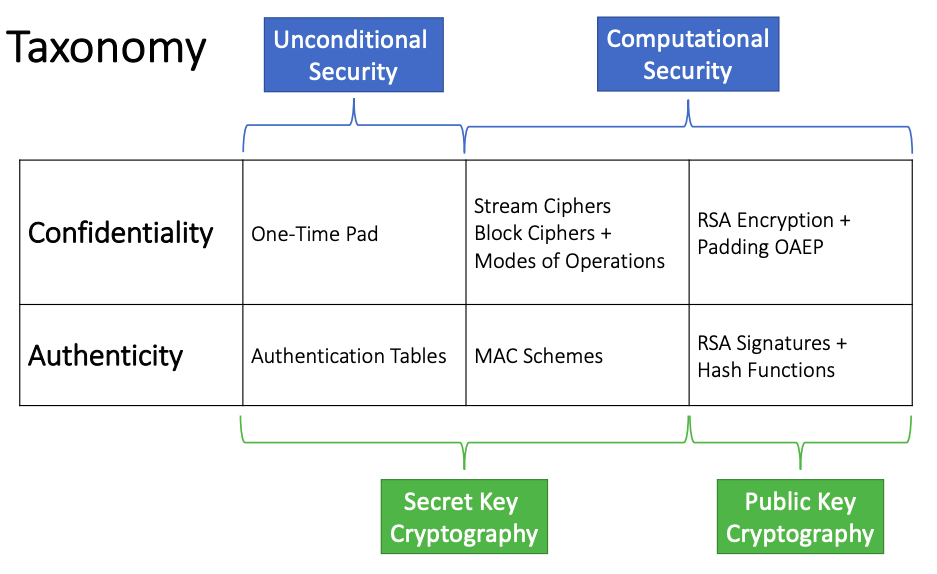
\includegraphics[width=\linewidth]{content/taxanomy.png}
}


%===================================
\section{Authentication, Secret-Key systems}

	\frame{\frametitle{Definition of security: Definition 6.1}
		Consider any adversary who runs in time much less than what exhaustive key search would take. The authentication scheme is secure if no such adversary can play the game specified above and in the end produce a message $m_0$ and a MAC $c_0$ such that $V_K(m_0, c_0) = \top$ and $m_0 \notin \{m_1, ... M_t\}$


		\textit{In more human language: even if the adversary has seen some number of messages with valid MACs, he still cannot come up with a message that was not sent and a valid MAC for that message. This is the case even if the adversary can choose the valid messages to be sent.}
	}

	\frame{\frametitle{Cipher Block Chaining MAC}
		\textbf{CBC-MAC}: If a Block Cipher, such as AES is secure, then it can be used to construct a MAC. \newline
		\textit{How is it built}: We encrypt the same message, but using an all-zero $IV$, and use the last block as the MAC. 
		\newline
		\textit{Intuition}: The last block depends on the input in a complicated way, and is therefore extremely difficult to forge. 
	}

    \frame{\frametitle{Cipher Block Chaining MAC}
        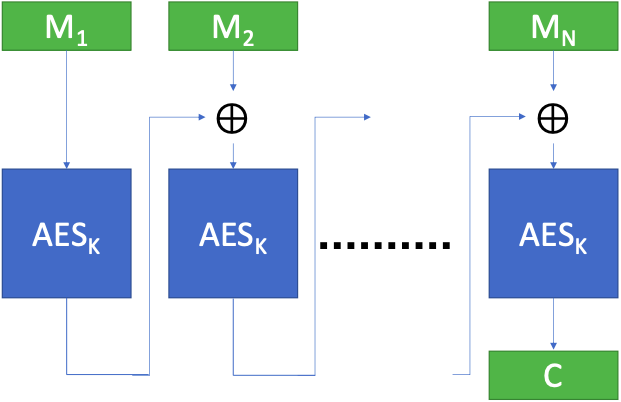
\includegraphics[width=\linewidth]{content/cbc-mac.png}
    }

	\frame{\frametitle{Authenticity}
		A secret-key system for Authentication consists of $3$ algorithms: $G, MAC, V$. $G$ generates a key, $MAC$ authenticates messages, $V$ verifies received messages. $G$ usually produces a key by just outputting a random bit string of fixed length. $MAC$ takes as input $m, K$ and outputs a $MAC$. $c = MAC_K(m)$. Then $m, c$ is sent who will run $V_K(m, c) = \{\top, \bot\}$. We require the following
		$$
			V_k(m, MAC_K(m)) = \top
		$$
	}
	
	\frame{\frametitle{Difference between signature and MAC}
		\begin{itemize}
			\item Secret Key schemes rely on all parties having the same keys. Only parties that have the key can be convinced that they are talking with each other, but they cannot convince others (who do not share the key)
			\item With public key schemes, everyone can verify the message because everyone is allowed to have the public key. 
		\end{itemize}
	}

	\frame{\frametitle{Why simplistic RSA signatures are not secure}
		\begin{itemize}
			\item RSA relies on the identity $s^e \text{ mod } n = (m^d \text{ mod } n)^e \text{ mod } n = m$
			\item But an adversary can choose an $s$ such that $m = s^e \text{ mod } n$
			\item Now $m$ would be a ``signed'' message
		\end{itemize}
	}

	\frame{\frametitle{Hash functions: Properties and examples}
		Hash functions can solve speed and security problems. Their desirable properties for hash functions are as follows
		\begin{itemize}
			\item Should take message of any length
			\item Should produce output of fixed length
			\item Speed similiar to secret-key systems
			\item Collisions should be hard to produce. That is, hard to find $x, y : x \neq y$ and $h(x) = h(y)$. 
		\end{itemize}
		Examples of hash functions in use are
			\begin{itemize}
				\item \textbf{SHA-256}: Produces 256-bit outputs
				\item \textbf{MD5}: Totally borken 
				\item \textbf{SHA-1}: Collisions have been found (Chosen Plaintext attack was discovered recently, now more broken)
			\end{itemize}
	}

	\frame{\frametitle{Hash-and-sign}
			Since hash functions typically produce output that is smaller than the input, cryptograhy on hashed inputs is typically faster. Since it is not computationally viable to produce collisions, it is hard to reverse the hash of a message. Therefore it is at least as convincing to sign a hash as the message itself. This leads to new algorithms
			\begin{itemize}
				\item $S'_{sk}(m) = S_{sk}(h(m))$
				\item $V'_{pk}(m, s) = V_{pk}(h(m), s)$
			\end{itemize}
			Now the previous attack still works, but having it sign forged messages is much harder. 
	}

	\subsection{Unconditional authentication}
		\frame{\frametitle{Table-based}
			For a finite number of messages, sender and receive agrees in advance on a table of t-bit MACs. Finding a correct MAC happens with probability $2^{-t}$. Finding a MAC requires guessing a random t-bit string. 
		}

\section{Authenticity, Public-Key Systems}
		\frame{\frametitle{Public-Key systems}
			Consists of $3$ algorithms, $G, S, V$. 
			\begin{itemize}
				\item S authenticates (signs)
				\item V verifies message (just like SK-case)
				\item G generates key pair
				\item $k_{sk}$ signs
				\item $k_{pk}$ is used to verify messages
				\item Requires distribution of public keys
			\end{itemize}
			}

			\frame{\frametitle{Definition 6.3: Definition of security}
				The adversary is given the public key \textit{pk}. He is allowed to specify any number of messages that he wants, say $m_1, ... m_t$. And he is given a valid authenticators $c_1 = S_{sk}(m1), ... c_t = S_{sk}(m_t)$ for these messages. The public-key authentication scheme is secure if the adversary cannot efficiently produce a message $m_0$ and an authenticator $c_0$ such that $V_{pk}(m_0, c_0) = \top$ and $m_0 \notin \{m_0, ..., m_t\}$.
			}

			\frame{\frametitle{Replay Attacks}
					A replay attack is when a message is intercepted, and is then sent again by an adversary. This means that even authenticated messages could be attacked. 
					Some remedies include
					\begin{itemize}
						\item Storing all the messages. Takes up a lot of space
						\item Store last seen message with a counter. This has problems if messages arrive late
						\item Have receiver send a nonce $R$ to sender. Send message + MAC computed from the message and nonce. 
					\end{itemize}
			}
			
		

\end{document}

